\documentclass{tum-book}

\renewcommand{\Titel}{Python User Interface for the mbsolve Project}
\renewcommand{\Author}{Mariem Kthiri}
\renewcommand{\Beschreibung}{\textbf{Report for Engineer Practice}\\ At the Faculty of Electrical Engineering and Information Technology at the Technical University of München.}
\renewcommand{\Extra}{
  \textbf{Supervised by}\\
  Michael Riesch, B.Sc.\\
  Professorship of Computational Photonics\\
  \vspace{12pt}
  \
  \textbf{Submitted on}\\
  München, 02.05.2017
}

\lstset{language=C,
  %captionpos=b,
  % CUDA specific keywords
  morekeywords={__global__, __device__, __host__, __shared__, real}
}

\usepackage{listings}
\usepackage[intoc,prefix]{nomencl}
\makeglossary
\makenomenclature

\begin{document}

\frontmatter

\let\cleardoublepage\clearpage

\tableofcontents

\mainmatter

\chapter{Introduction}
\label{chapter:introduction}

Quantum cascade laser is a type of semiconductor emitting mid-infrared portion of electromagnetic spectrum. This frequency range allows a multitude of applications especially in the field of spectroscopy where it serves the detection of toxic chemicals, explosives, and drugs. In this context, the mbsolve Project provides the required simulation relying on C++ programming with a Python user interface. This Engineer's practice aims at the design of this interface.\\
Chapter \ref{chapter:theory} provides the theoretical background and starting point. In chapter \ref{chapter:conception}, the conception and realisation of the project will be described and detailed. The outcome is presented in chapter \ref{chapter:results}. The discussion of the results concludes this work.






\chapter{Theoretical Background}
\label{chapter:theory}

\setlength\parindent{12pt} In this project,a high performing programming language was required for the simulation because of the large size of data and the elaborate numerical treatments. C++ fullfills these criteria not to mention that it is available everywhere and reasonably well standardized. Nevertheless it has some drawbacks: First of all it is not interactive and implementing it for user-interfaces (especially graphic user interfaces) can be quite complex. That is why it was opted for Python for the interface which brings flexibilty interactivity and simplicity(see Tab.~\ref{table:settings}).\\
To sum it up, the goal is to create a common interface that enables the user to wrap different C++ libraries in Python modules and load them dynamically during the execution of the program.\\



\begin{table}[htb]
\centering
\begin{tabular}{|cc|}
\hline
\textbf{C++} & \textbf{Python}\\
\hline
\textbf{Advantages} & \textbf{Advantages} \\
High performance and speed & Flexibility (fast edit-build-debug cycle)
\\useful for intensive tasks & Interactivity\\

Parallelization techniques & (create, change, view objects at runtime) \\

\textbf{Drawbacks} & \textbf{Drawbacks} \\

Non-interactive & relatively slow\\
Writing user-interfaces & Limitations with memory intensive tasks\\
is complex &  Limitations with database access\\
\hline
\end{tabular}
\caption{Characterictics of C++ and Python.\label{table:settings}}

\end{table}

\chapter{Conception and Realisation}
\label{chapter:conception}

\section{Literature and basics}
At the beginning, it was necessary to acquire some basics about quantum mechanics (density matrix, Maxwell-Bloch equations..) by reading some introductory literature ~\cite{tang2005}. A concrete example for the simulation and the numerical solving of the Maxwell-Bloch system was described in the paper of Ziolkowski.\\
QuTiP, a Python Toolbox for simulating the dynamics of open quantum systems, was then the starting point. It offered a variety of examples using Jupyter Notebooks: an interactive tool designed to display neatly arranged code blocks with human-friendly text which makes project easier to manage and share, they are used in this case to describe quantum mechanic systems, such as single-atom lasing, quantum Monte Carlo trajectories...\\
\section{Python/C++ Interface}
Creating the Python/C++ Interface was possible through different means:\\
\begin{itemize}
\item Boost.Python: Boost.Python is an open source C++ library which provides an interface for binding C++ classes and functions to Python. But it is bound to GCC which leads to a huge dependance and its extensive use of C++ template can cause compilation problems and the consumption of a large amount of memory. \\
\item ctpyes: ctypes is a foreign library for Python, that allows calling DLLs or shared libraries and wrapping them in Python modules. It is a convenient way to reach for a few functions within a DLL, but not to make large C++ libraries available to Python in performance-critical situations.\\
\item SWIG (Simplified Wrapper and Interface Generator): It is a language neutral compiler that turns C/C++ declarations into scripting language interfaces. It targets Python, Tcl, Perl, MATLAB, etc.. One of its important features is that it is simple and completely automated. In fact, it creates two different files; a C/C++ source file (module\textunderscore name)\textunderscore wrap.c or (module\textunderscore name)\textunderscore wrap.cxx and a Python source file (module\textunderscore name).py. The first one needs to be compiled and linked with the rest of the C/C++ library to create an extension module. The second one is the file that will be imported in Python(see Fig.\ref{fig:swig}).\\
\begin{figure}[htb]
  \centering
  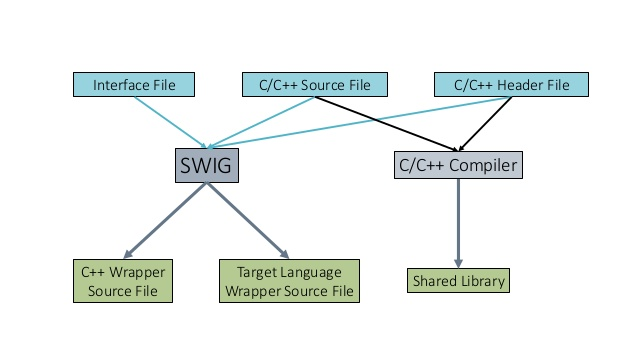
\includegraphics[width=0.5\textwidth]{figures/swig_func}
  \caption{Functionality of SWIG} ~\cite{swig}
  \label{fig:swig}
\end{figure}
\end{itemize}
After installing SWIG, a Python module was created starting from an interface file and a header file written in C++. The next step was to wrap a C++ class in order to create instances of this class and modify its attributes in the Python Testprogram. Then the complete C++ library was gradually elaborated, adding each time required attributes and declarations.\\
\section{Serialisation of input parameters}
The next point to handle was the input parameters, how to extract them from an XML File and then store them with results at the end. The first option was to use exml or lxml libraries, which could parse XML files but the resulting objects having NoType made handling them problematic. Therefore, a simple object-XML mapper for Python called dexml was applied to serialize the metadata by defining subclasses of the class dexml.Model and saving the parameters as instances.\\
\section{Storing results}
Furthermore, it was necessary to specify the file format for the simulation results, which lead to the following options:\\
\begin{itemize}
\item XML (Extensible Markup Language): XML's biggest advantage is that it provides developers with a tool that concisely and unambiguously defines the format of data records. However it is not suitable for large amount of data.\\
\item VTK (Visualization Toolkit): It is a powerful tool to visualize scalars, vectors, complex numbers.. but  requires a diffcult setup and an understanding of the framework.\\ 
\item HDF5 (Hierarchical Data Format): HDF5 is a file format that enables the storage and management of data of different types. It is suitable for high volume and complex data. In fact, a HDF5 file consists of datasets (multidimensional arrays) and groups, which contain diverse data: datasets, graphics, other groups.. Another advantage is the ability of compression and chunking, which makes the storage more flexible and efficient ~\cite{hdf5}.\\ 
\end{itemize}
All that considered, HDF5 is the most suitable file format not only to store large amount of data (results) but also different types simultaneously (Metadata).
\section{Git}
After settling the C++ library that contains all the necessary classes and functions, using SWIG to incorporate it in Python, choosing dexml for serialisation of metadata and HDF5 for storage of results, a Git project was created to gather all the pieces, register every step of the realisation and facilitate data exchange and work coordination between me and my supervisor. \\
\section{Makefile/CMake}
To get more experience in handling scientific projects, it was extremely efficient to understand the process of Makefiles and then CMake and apply them on my work. both aim at building executable programs starting from many modules.
\begin{itemize}
\item Makefiles are a simple way to organize code compilation, they consist of a list of target entries, where it is specified for each target the dependencies needed as well as the command line to apply. Besides it only rebuilds in case of new modules added to the program.
\item CMake is a cross platform build system, that automatically generates Makefiles using the CMakeListst.txt file, that specifies the packages, libraries, source files,.. needed to build.
\end{itemize}  


\chapter{Results}
\label{chapter:results}
Most of the work was realised on Linux and delivered the required Interface consisting of different parts.
\section{Python/C++ Interface}
\subsection{Source files} 
These include the interface file, needed by SWIG, the header file, declaring the classes and functions as well as the C++ source code.
\begin{itemize}
\item C++ Class Record: specifies which results should be stored and in which interval.
\item C++ Class Material: contains the characteristics of each material (name, electric permittivity, magnetic permeability).
\item C++ Class Region: includes the specifications of each region (name, start, end, material index).
\item C++ Class Device: lists the materials and regions applied in the simulation.
\item C++ Class Scenario: contains the total time of the simulation, the timestep and the list of the records.
\item C++ Class Result: gives a vector of values corresponding to the measured result (electric field, elements of the density matrix)
\item C++ Function: Depending on the device and scenario, calculates the results.
\end{itemize}

\subsection{CMakeLists file}
SWIG can be incorporated in many build systems, in this case CMake, which can detect the SWIG executable and find the required packages and libraries for linking in order to build shared libraries. Using a single cross platform file (CMakeLists.txt) and two simple commands: cmake and make, CMake generates native build files such as makefiles, nmake files and Visual Studio projects which call SWIG and compile the generated C++ files into shared objects (.so for UNIX or .pyd for Windows).

\subsection{Python Testprogram}
The testprogram (available as a skript and a notebook) allows the setup of materials, sevice, Scenario etc., extracts metadata from an XML file, calls the C++ function that calculates the required results, displays them and  stores them in addition to the metadata in a HDF5 File.\\

To run the program, the user can clone the project from Github, create a build directory and run the commands: cmake.. and make, this will generate all the necessary files to compile and link in the same folder. Afterwards the testprogram must be brought and run through: python project.py. 

Moreover, it was seeked to make the project as flexible as possible, or in other words compatible with different versions of Python as well as realisable on variable operating systems.
\section{Compatibility with Python3}
SWIG is compatible with the different versions of Python (Python 2.7 and Python 3.x). To choose a specific version, all that has to be done is to indicate it in the command line of compiling with cmake, which will find the corresponding packages and libraries and use them to compile and link. As an example, here are the both possibilities to compile on Linux with:
\begin{itemize}
\item \textbf{Python 2.7} 
cmake .. -DPYTHON\textunderscore LIBRARIES=/usr/lib/python2.7
make
python project.py
\item \textbf{Python 3} 
cmake .. -DPYTHON\textunderscore LIBRARIES=/usr/lib/python3
make
python3 project.py
\end{itemize}

\section{SWIG on Windows}
Another approach is available on Windows: building the extension module using a configuration file (conventionally called setup.py), it creates an extension module object using the source code files generated by swig, in addition to the original C++ source and compiles it into a shared object file or DLL (.pyd on Windows), which can be called in the testprogram. 




\chapter{Conclusion}

The Python/C++ Interface is estimated to be the most suitable way to combine the efficiency and performance of C++ programming with the flexibility and interactivity of Python. SWIG was implemented to automatically create the wrappers needed to access the C++ Library from Python. Nevertheless, there are other possibilities to achieve this goal, such as Cython which is a Python like language for writing C/C++ extensions. In addition, further optimizations can be seeked on Windows using Visual Studio.


\bibliographystyle{osajnl}
\bibliography{literature}

\end{document}
